\documentclass[12pt, a4paper, onecolumn]{IEEEtran}
\usepackage[utf8]{inputenc}
\usepackage{graphicx}
\usepackage{amsmath}
\usepackage{listings}
\usepackage{xcolor}
\graphicspath{ {img/} }
\title{%
    Independent Component Analysis \\
  \large Term paper ( Tutorial ) Advanced Digital Signal Processing }
\author{Pin-Chun Hsu(B03901023), Prof. Jian-Jiun Ding}
\begin{document}

\maketitle
\section{abstract}
This tutorial presents an introduction to independent component analysis (ICA). Unlike principal component analysis, which is based on the assumptions of uncorrelatedness and  normality,  ICA  is  rooted  in  the  assumption  of  statistical  independence. Foundations and basic knowledge necessary to understand the technique are provided hereafter. Also included is a short  tutorial illustrating the implementation of two ICA algorithms (FastICA and InfoMax) with the use of the Mathematica software.
\section{introduction}

Imagine that you are in a room where two people are speaking simultaneously. You have two microphones, which you hold in different locations. The microphones give you two recorded time signals, which we could denote by $x_1(t)$ and $x_2(t)$, with $x_1$ and $x_2$ the amplitudes, and $t$ the time index. Each of these recorded signals is a weighted sum of the speech signals emitted by the two speakers, which we denote by $s_1(t)$ and $s_2(t)$. We could express this as a linear equation:
\begin{equation}
x_1(t) = a_{11}s_1 + a_{12}s_2
\end{equation}
\begin{equation}
x_2(t) = a_{21}s_1 + a_{22}s_2
\end{equation}
where $a_{11}$,$a_{12}$,$a_{21}$, and $a_{22}$ are some parameters that depend on the distances of the microphones from the speakers. It would be very useful if you could now estimate the two original speech signals $s_1(t)$ and $s_2(t)$, using only the recorded signals $x_1(t)$ and $x_2(t)$. This is called the cocktail-party problem. For the time being, we omit any time delays or other extra factors from our simplified mixing model.

\begin{figure}[h]
    \centering
    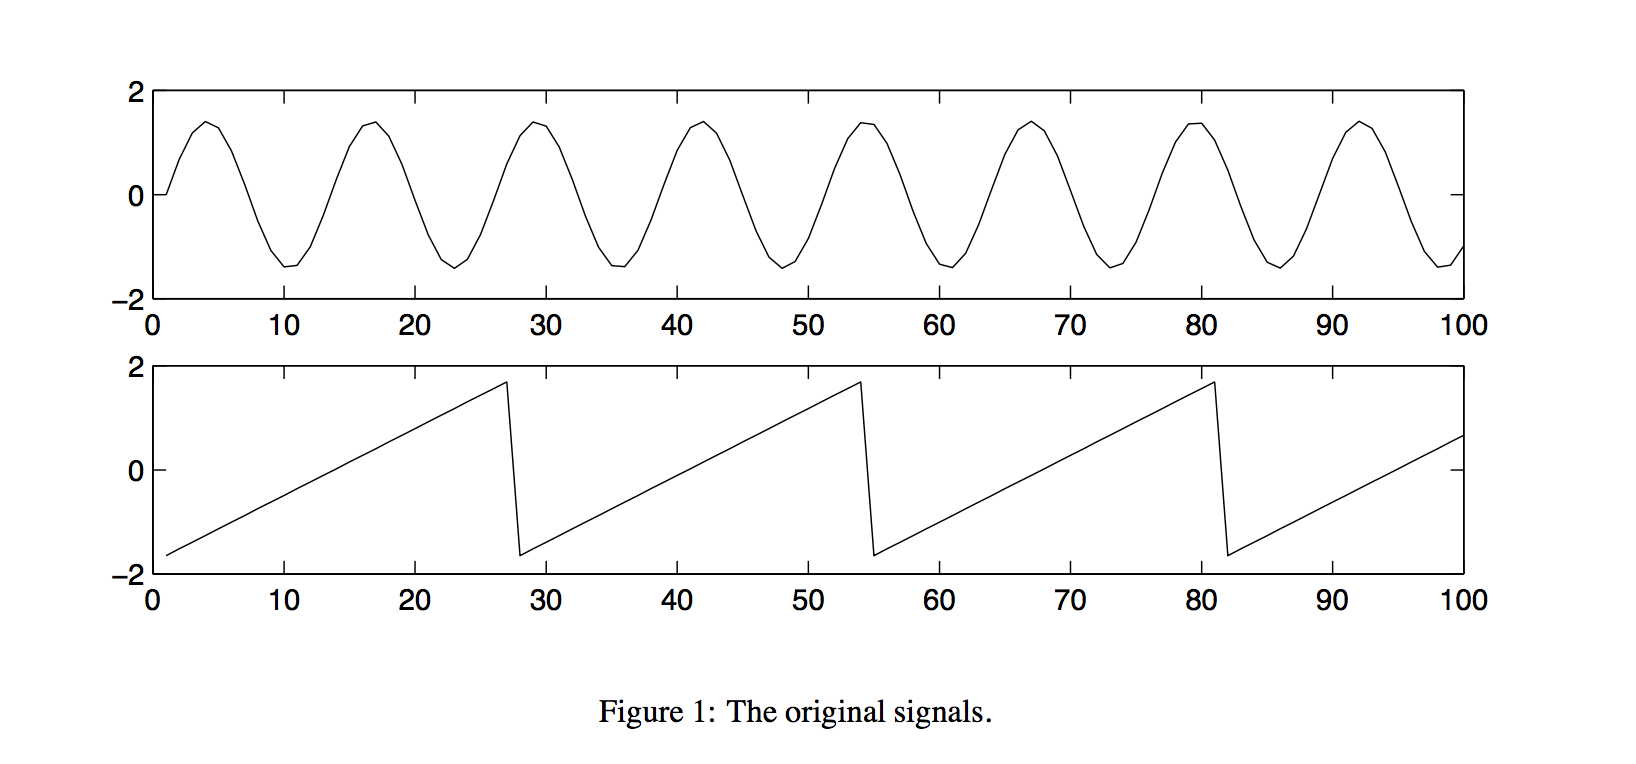
\includegraphics[width=1\textwidth]{1}
\end{figure}
As an illustration, consider the waveforms in Fig. 1 and Fig. 2. These are, of course, not realistic speech signals, but suffice for this illustration. The original speech signals could look something like those in Fig. 1 and the mixed signals could look like those in Fig. 2. The problem is to recover the data in Fig. 1 using only the data in Fig. 2.
Actually, if we knew the parameters $a_{ij}$, we could solve the linear equation in (1) by classical methods. The point is, however, that if you don’t know the $a_{ij}$, the problem is considerably more difficult.
One approach to solving this problem would be to use some information on the statistical properties of the signals $s_i{t}$ to estimate the aii. Actually, and perhaps surprisingly, it turns out that it is enough to assume that $s_1(t)$ and $s_2(t)$, at each time instant t, are statistically independent. This is not an unrealistic assumption in many cases, and it need not be exactly true in practice.
\begin{figure}[h]
    \centering
    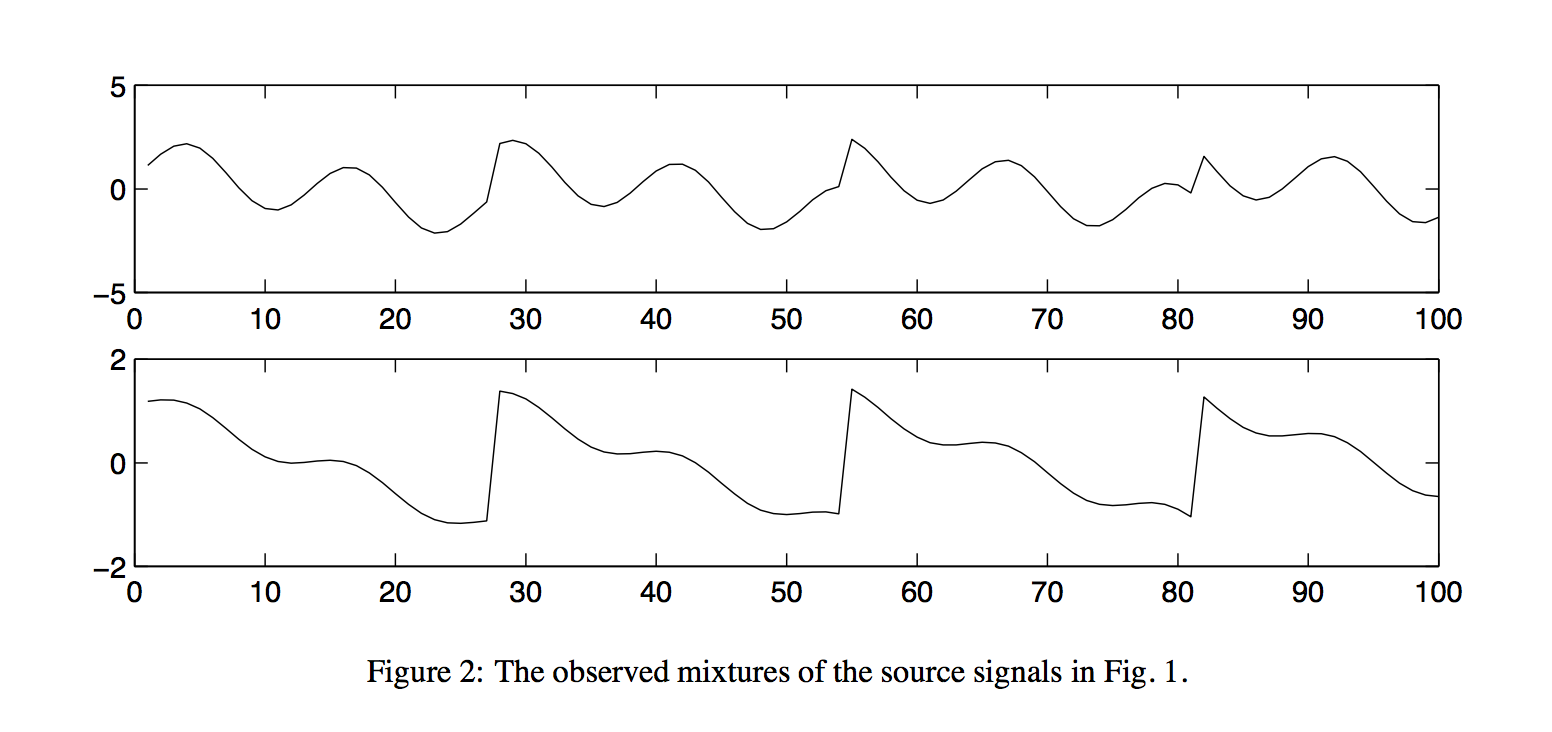
\includegraphics[width=1\textwidth]{2}
\end{figure}
The recently developed technique of Independent Component Analysis, or ICA, can be used to estimate the ai j based on the information of their independence, which allows us to separate the two original source signals $s_1(t)$ and $s_2(t)$ from their mixtures $x_1(t)$ and $x_2(t)$. Fig. 3 gives the two signals estimated by the ICA method. As can be seen, these are very close to the original source signals (their signs are reversed, but this has no significance.)
Independent component analysis was originally developed to deal with problems that are closely related to the cocktail-party problem. Since the recent increase of interest in ICA, it has become clear that this principle has a lot of other interesting applications as well.

\begin{figure}[h]
    \centering
    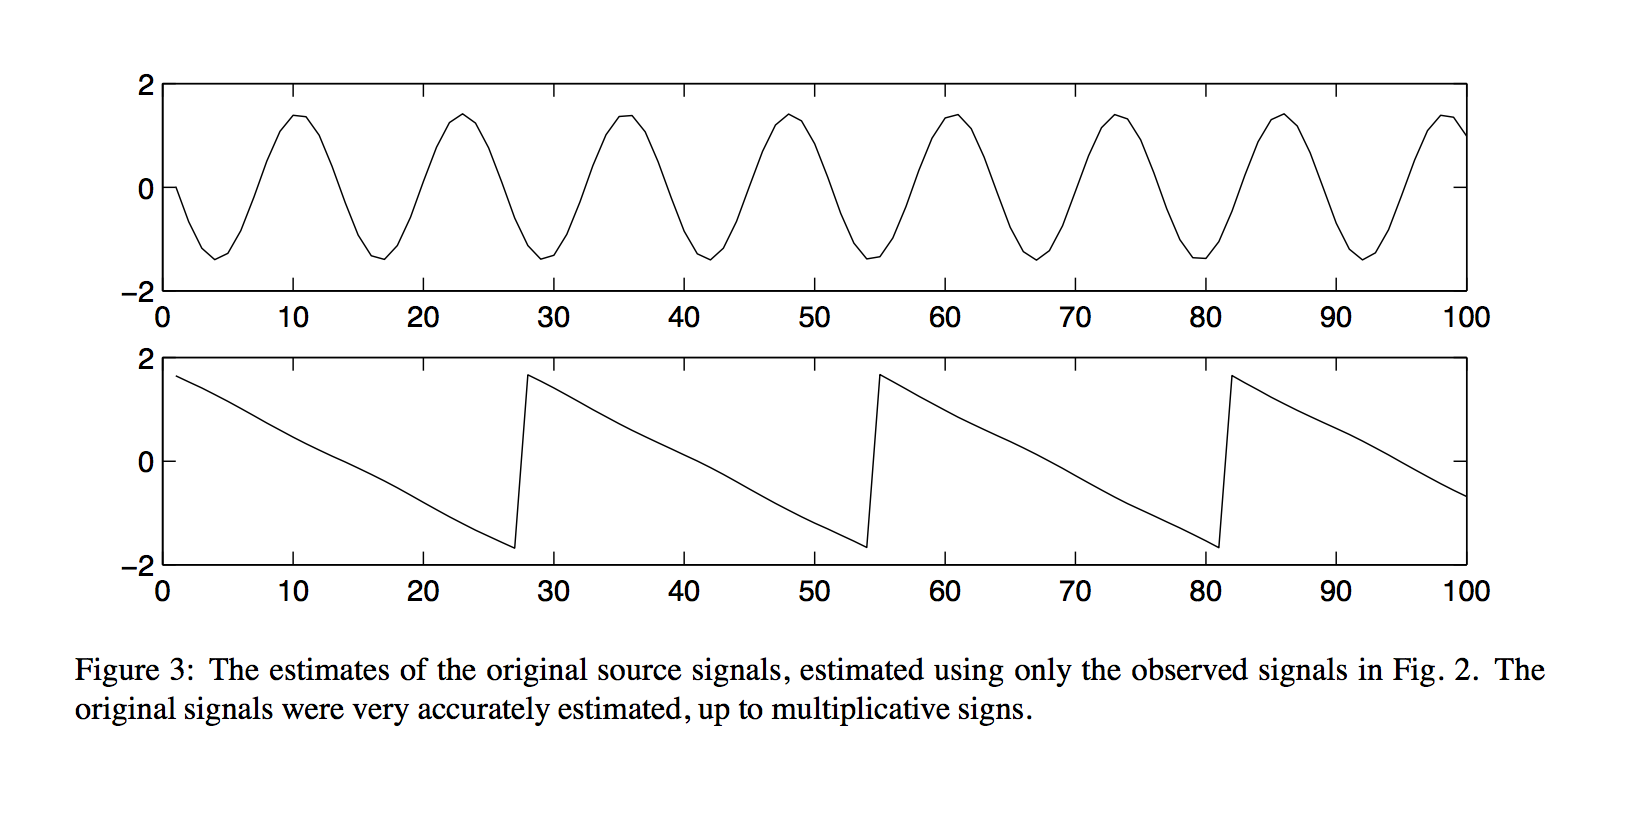
\includegraphics[width=1\textwidth]{3}
\end{figure}
Consider, for example, electrical recordings of brain activity as given by an electroencephalogram (EEG). The EEG data consists of recordings of electrical potentials in many different locations on the scalp. These potentials are presumably generated by mixing some underlying components of brain activity. This situation is quite similar to the cocktail-party problem: we would like to find the original components of brain activity, but we can only observe mixtures of the components. ICA can reveal interesting information on brain activity by giving access to its independent components.
Another, very different application of ICA is on feature extraction. A fundamental problem in digital signal processing is to find suitable representations for image, audio or other kind of data for tasks like compression and denoising. Data representations are often based on (discrete) linear transformations. Standard linear transforma- tions widely used in image processing are the Fourier, Haar, cosine transforms etc. Each of them has its own favorable properties (Gonzales and Wintz, 1987).
It would be most useful to estimate the linear transformation from the data itself, in which case the transform could be ideally adapted to the kind of data that is being processed.

\begin{figure}[h]
    \centering
    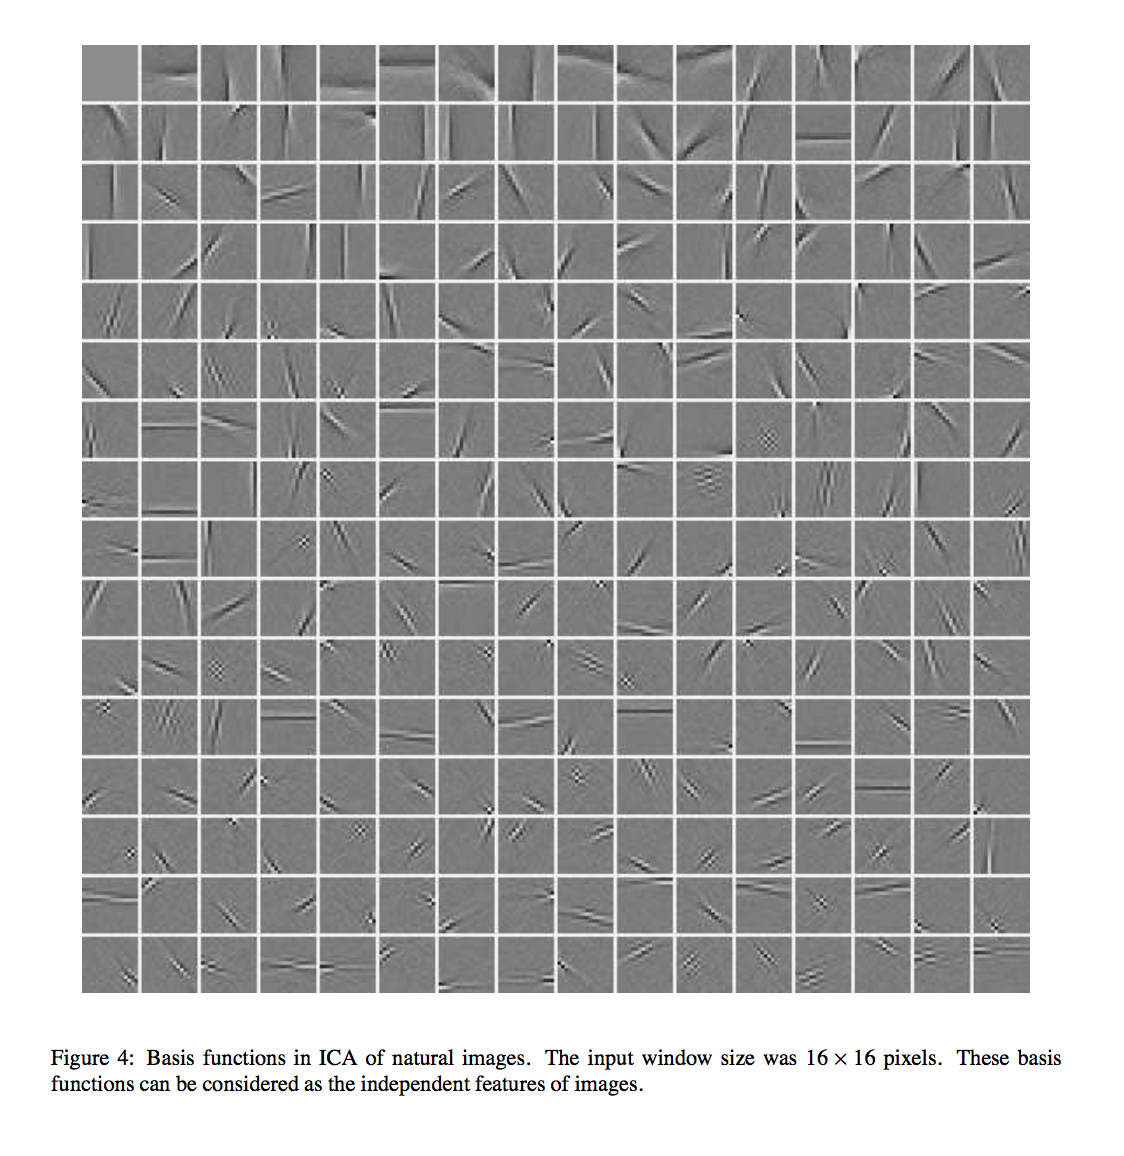
\includegraphics[width=1\textwidth]{4}
\end{figure}
Figure 4 shows the basis functions obtained by ICA from patches of natural images. Each image window in the set of training images would be a superposition of these windows so that the coefficient in the superposition are independent. Feature extraction by ICA will be explained in more detail later on.
All of the applications described above can actually be formulated in a unified mathematical framework, that of ICA. This is a very general-purpose method of signal processing and data analysis.
\section{definition}
To rigorously define ICA (Jutten and Hérault, 1991; Comon, 1994), we can use a statistical “latent variables” model. Assume that we observe $n$ linear mixtures $x_1,...,x_n$ of $n$ independent components, for all j,

\begin{equation}
    x_j = a_{j1}s_1 + a_{j2} + s_2 +...+ a_{jn}s_n
\end{equation}
We have now dropped the time index $t$; in the ICA model, we assume that each mixture $x_j$ as well as each independent component $s_k$ is a random variable, instead of a proper time signal. The observed values $x_j(t)$, e.g., the microphone signals in the cocktail party problem, are then a sample of this random variable. Without loss of generality, we can assume that both the mixture variables and the independent components have zero mean: If this is not true, then the observable variables $x_i$ can always be centered by subtracting the sample mean, which makes the model zero-mean.
It is convenient to use vector-matrix notation instead of the sums like in the previous equation. Let us denote by $x$ the random vector whose elements are the mixtures $x_1,...,x_n$, and likewise by $s$ the random vector with elements $s_1,...,s_n$. Let us denote by $\mathbf{A}$ the matrix with elements $a_{ij}$. Generally, bold lower case letters indicate vectors and bold upper-case letters denote matrices. All vectors are understood as column vectors; thus $x_T$ , or the transpose of $\mathbf{x}$, is a row vector. Using this vector-matrix notation, the above mixing model is written as
\begin{equation}
\mathbf{x}=\mathbf{As}.
\end{equation}
Sometimes we need the columns of matrix $\mathbf{A}$; denoting them by $\mathbf{a}_j$ the model can also be written as
\begin{equation}
\mathbf{x} = \sum_{i=1}^{n}\mathbf{a}_is_i
\end{equation}
The statistical model in Eq. 4 is called \textbf{independent component analysis, or ICA model}. The ICA model is a generative model, which means that it describes how the observed data are generated by a process of mixing the components $s_i$. The independent components are latent variables, meaning that they cannot be directly observed. Also the mixing matrix is assumed to be unknown. All we observe is the random vector $\mathbf{x}$, and we must estimate both $\mathbf{A}$ and $\mathbf{s}$ using it. This must be done under as general assumptions as possible.
The starting point for ICA is the very simple assumption that the components si are statistically independent. Statistical independence will be rigorously defined in Section 3. It will be seen below that we must also assume that the independent component must have nongaussian distributions. However, in the basic model we do not assume these distributions known (if they are known, the problem is considerably simplified.) For simplicity, we are also assuming that the unknown mixing matrix is square, but this assumption can be sometimes relaxed, as explained in Section 4.5. Then, after estimating the matrix $\mathbf{A}$, we can compute its inverse, say $\mathbf{W}$, and obtain the independent component simply by:
\begin{equation}
    \mathbf{s=Wx}
\end{equation}
ICA is very closely related to the method called blind source separation (BSS) or blind signal separation. A “source” means here an original signal, i.e. independent component, like the speaker in a cocktail party problem. “Blind” means that we no very little, if anything, on the mixing matrix, and make little assumptions on the source signals. ICA is one method, perhaps the most widely used, for performing blind source separation.
In many applications, it would be more realistic to assume that there is some noise in the measurements (see e.g. (Hyvärinen, 1998a; Hyvärinen, 1999c)), which would mean adding a noise term in the model. For simplicity, we omit any noise terms, since the estimation of the noise-free model is difficult enough in itself, and seems to be sufficient for many applications.

\section{Ambiguities of ICA}
In the ICA model in Eq. (4), it is easy to see that the following ambiguities will hold: 1. We cannot determine the variances (energies) of the independent components.
The reason is that, both $s$ and $\mathbf{A}$ being unknown, any scalar multiplier in one of the sources $s_i$ could always be cancelled by dividing the corresponding column $a_i$ of $\mathbf{A}$ by the same scalar; see eq. (5). As a consequence, we may quite as well fix the magnitudes of the independent components; as they are random variables, the most natural way to do this is to assume that each has unit variance: $E{s_{2i}} = 1$. Then the matrix $\mathbf{A}$ will be adapted in the ICA solution methods to take into account this restriction. Note that this still leaves the ambiguity of the sign: we could multiply the an independent component by $−1$ without affecting the model. This ambiguity is, fortunately, insignificant in most applications.

2. We cannot determine the order of the independent components.
The reason is that, again both $s$ and $\mathbf{A}$ being unknown, we can freely change the order of the terms in the sum in (5), and call any of the independent components the first one. Formally, a permutation matrix $\mathbf{P}$ and its inverse can be substituted in the model to give $\mathbf{x = AP^{−1}Ps}$. The elements of Ps are the original independent variables $s_j$, but in another order. The matrix $\mathbf{AP^−1}$ is just a new unknown mixing matrix, to be solved by the ICA algorithms.
\section{Illustration of ICA}
To illustrate the ICA model in statistical terms, consider two independent components that have the following
uniform distributions:
\begin{equation}
    \ p(s_i) =
      \begin{cases}
        \frac{1}{2\sqrt{3}}       & \quad \text{if } \abs{s_i} \leq \sqrt{3}\\
        0  & \quad \text{otherwise}\\
      \end{cases}
    \
\end{equation}
The range of values for this uniform distribution were chosen so as to make the mean zero and the variance equal to one, as was agreed in the previous Section. The joint density of $s_1$ and $s_2$ is then uniform on a square. This follows from the basic definition that the joint density of two independent variables is just the product of their marginal densities (see Eq. 10): we need to simply compute the product.
\begin{figure}[h]
    \centering
    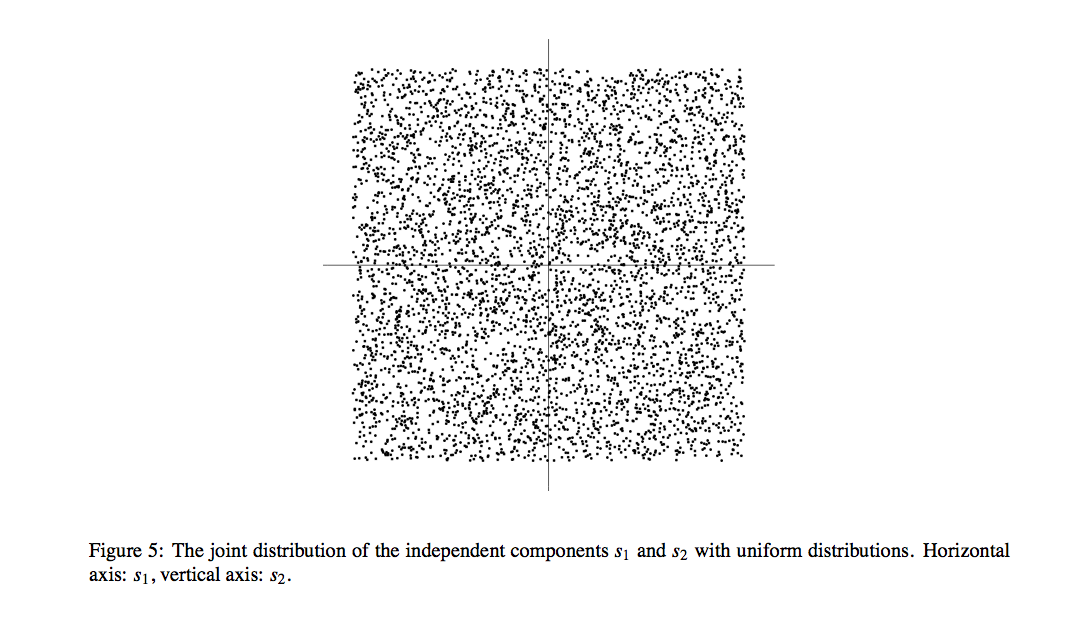
\includegraphics[width=1\textwidth]{5}
\end{figure}

The joint density is illustrated in Figure 5 by showing data points randomly drawn from this distribution. Now let as mix these two independent components. Let us take the following mixing matrix:
\begin{equation}
    \ \mathbf{A}_{0} =
     \begin{pmatrix}
      2 & 2\\
      3 & 1
     \end{pmatrix}
     \
\end{equation}
This gives us two mixed variables, $x_1$ and $x_2$. It is easily computed that the mixed data has a uniform distribution on a parallelogram, as shown in Figure 6. Note that the random variables $x_1$ and $x_2$ are not independent any more; an easy way to see this is to consider, whether it is possible to predict the value of one of them, say $x_2$, from the value of the other. Clearly if $x_1$ attains one of its maximum or minimum values, then this completely determines the value of $x_2$. They are therefore not independent. (For variables $s_1$ and $s_2$ the situation is different: from Fig. 5 it can be seen that knowing the value of $s_1$ does not in any way help in guessing the value of $s_2$.)
The problem of estimating the data model of ICA is now to estimate the mixing matrix $\mathbf{A}_0$ using only information contained in the mixtures $x_1$ and $x_2$.

\begin{figure}[h]
    \centering
    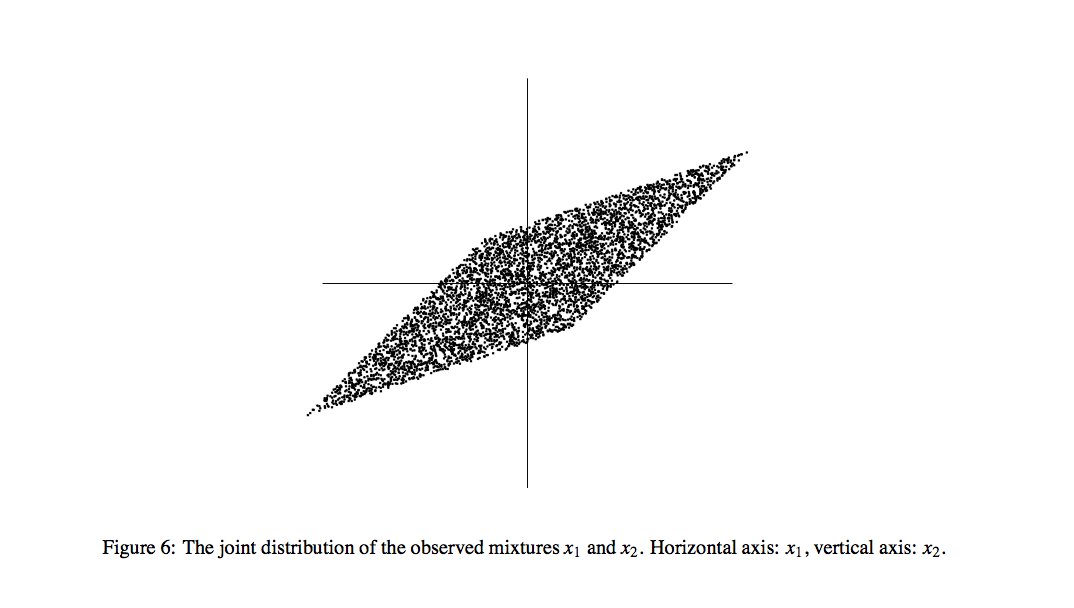
\includegraphics[width=1\textwidth]{6}
\end{figure}
Actually, you can see from Figure 6 an intuitive way of estimating $\mathbf{A}$: The edges of the parallelogram are in the directions of the columns of $\mathbf{A}$. This means that we could, in principle, estimate the ICA model by first estimating the joint density of $x_1$ and $x_2$, and then locating the edges. So, the problem seems to have a solution.
In reality, however, this would be a very poor method because it only works with variables that have exactly uniform distributions. Moreover, it would be computationally quite complicated. What we need is a method that works for any distributions of the independent components, and works fast and reliably.
\section{ICA and Projection Pursuit}
It is interesting to note how our approach to ICA makes explicit the connection between ICA and projection pursuit. Projection pursuit (Friedman and Tukey, 1974; Friedman, 1987; Huber, 1985; Jones and Sibson, 1987) is a technique developed in statistics for finding “interesting” projections of multidimensional data. Such projections can then be used for optimal visualization of the data, and for such purposes as density estimation and regression. In basic (1-D) projection pursuit, we try to find directions such that the projections of the data in those directions have interesting distributions, i.e., display some structure. It has been argued by Huber (Huber, 1985) and by Jones and Sibson (Jones and Sibson, 1987) that the Gaussian distribution is the least interesting one, and that the most interesting directions are those that show the least Gaussian distribution. This is exactly what we do to estimate the ICA model. The projection on the first principal component (vertical), on the other hand, fails to show this structure.
Thus, in the general formulation, ICA can be considered a variant of projection pursuit. All the nongaussianity measures and the corresponding ICA algorithms presented here could also be called projection pursuit “indices” and algorithms. In particular, the projection pursuit allows us to tackle the situation where there are less indepen- dent components si than original variables xi is. Assuming that those dimensions of the space that are not spanned by the independent components are filled by gaussian noise, we see that computing the nongaussian projection pursuit directions, we effectively estimate the independent components. When all the nongaussian directions have been found, all the independent components have been estimated. Such a procedure can be interpreted as a hybrid of projection pursuit and ICA.
However, it should be noted that in the formulation of projection pursuit, no data model or assumption about independent components is made. If the ICA model holds, optimizing the ICA nongaussianity measures produce independent components; if the model does not hold, then what we get are the projection pursuit directions.

\section{Formulation of the Problem}

A typical example is the ``cocktail party problem''. Given
the signals $x_j(t)$ from $m$ microphones recording $n$ speakers in the
room ($m\ge n$), one wants to recover the voice $s_i(t)$ of each speaker.
The problem can be formulated as
\begin{itemize}
\item {\bf Given}
\[	x_i(t)=\sum_{j=1}^n a_{ij} s_j(t)\;\;\;\;\;(i=1,\cdots,m) \]
or in matrix form
\[	\left[ \begin{array}{c} x_1 \\ \cdots \\ x_m \end{array} \right]=
	\left[ \begin{array}{ccc} a_{11} & \cdots & a_{1n} \\
	\cdots & \cdots & \cdots \\ a_{n1} & \cdots & a_{mn}
\end{array} \right]
\left[ \begin{array}{c} s_1 \\ \cdots \\ s_n \end{array} \right]
\;\;\;\;\;\;\;\mbox{or}\;\;\;\;\;\;\;	{\mathbf x=As}	\]
\item {\bf Find}
\begin{itemize}
\item the estimation ${\mathbf y=Wx}$ of the source variables $s_j(t)$
	{\em the independent components},
\item and the linear combination matrix ${\mathbf A}$.
\end{itemize}
\end{itemize}
This is a blind source separation (BSS) problem, i.e., to separate
linearly mixed source signals. The word ``blind'' means that we do
not assume any prior knowledge about sources ${\mathbf s}$ or the mixing
process ${\mathbf A}$ except that the source signals $s_i$ are statistically
independent.

Although this BSS problem seems severely under constrained, the independent
component analysis (ICA) can find nearly unique solutions satisfying
certain properties.

ICA can be compared with
\htmladdnormallink{{\em principal component analysis} (PCA)}{../pca/index.html}
for decorrelation.  Given a set of variables ${\mathbf x}$, PCA finds a
matrix ${\mathbf W}$ so that the components of ${\mathbf y=Wx}$ are
uncorrelated. Only under the special case when ${\mathbf y}=[y_1,\cdots,y_n]$
are gaussian, are they also independent. In comparison, ICA is a more powerful
method in the senese that it satisfies a stronger requirement of finding
${\mathbf W}$ so that the components of ${\mathbf y=Wx}$ are independent
(and therefore are also necessarily uncorrelated).

\section{Methods of ICA Estimations}

\subsection*{Non-Gaussianity is Independence}

The theoretical foundation of ICA is the
\textbf{Central Limit Theorem},
which states that the distribution of the sum (average or linear
combination) of $N$ independent random variables approaches Gaussian
as $N\rightarrow \infty$. For example, the face value of a dice has a
uniform distribution from 1 to 6. But the distribution of the sum of a
pair of dice is no longer uniform. It has a maximum probability at the
mean of 7. The distribution of the sum of the face values will be better
approximated by a Gaussian as the number of dice increases.

Specifically, if $x_i$ are random variables independently drawn from an
arbitrary distribution with mean $\mu$ and variance $\sigma^2$. Then the
distribution of the mean $x=\sum_{i=1}^N x_i/N$ approaches Gaussian with
mean $\mu$ and variance $\sigma^2/N$.

To solve the BSS problem, we want to find a matrix ${\mathbf W}$ so that
${\mathbf y=Wx=WAs \approx s}$ is as close to the independent sources
${\mathbf s}$ as possible. This can be seen as the reverse process of the
central limit theorem above.

Consider one component $y_i={\mathbf w_i^TAs}$ of ${\mathbf y}$, where
${\mathbf w_i^T}$ is the ith row of ${\mathbf W}$. As a linear combination
of all components of ${\mathbf s}$, $y_i$ is necessarily more Gaussian
than any of the components unless it is equal to one of them (i.e.,
${\mathbf w_i^TA}$ has only one non-zero component.
In other words, the goal ${\mathbf y \approx s}$ can be achieved by finding
${\mathbf W}$ that maximizes the {\bf non-Gaussianity} of
${\mathbf y=Wx=WAs}$ (so that ${\mathbf y}$ is least Gaussian). This is
the essence of all ICA methods. Obviously if all source variables are
Gaussian, the ICA method will not work.

Based on the above discussion, we get requirements and constrains for the
ICA methods:

\begin{itemize}
\item The number of observed variables $m$ must be no fewer than the number
	of independent sources $n$ (assume $m=n$ in the following).
\item The source components are stochastically independent, and have to be
	non-Gaussian (with possible exception of at most one Gaussian).
\item The estimation of $A$ and $S$ is up to a scaling factor $c_i$.
	Let ${\mathbf C}=diag(c_1,\cdots,c_n)$ and ${\mathbf C}^{-1}=
	diag(1/c_1,\cdots,1/c_n)$,
	and ${\mathbf A}'={\mathbf AC}^{-1}$ and ${\mathbf s'=Cs}$, we have
\[	{\mathbf x=As=[AC^{-1}][Cs]=A's'}	\]
	Also the scaling factor $c_i$ could be either positive or negative.
	For this reason, we will always assume the independent components
	have unit variance $E\{s_i^2\}=1$. As they are also uncorrelated
	(all independent variables are uncorreclated), we have
	$E\{s_is_j\}=\delta_{ij}$, i.e.,
\[	E\{SS^T\}=I	\]
\item The estimated independent components are not in any particular
	order. When the order of the corresponding elements in both
	${\mathbf s}$ and ${\mathbf A}$ is rearranged, ${\mathbf x=As}$
	still holds.
\end{itemize}

All ICA methods are based on the same fundamental approach of finding a
matrix ${\mathbf W}$ that maximizes the non-Gaussianity of ${\mathbf s=Wx}$
thereby minimizing the independence of $S$, and they can be formulated as:
\[ {\bf
\mbox{ICA method}=\mbox{objective function}+\mbox{optimization algorithm}
} \]
All ICA methods are an optimization process (always iterative) to find a
matrix ${\mathbf W}$ to maximize some objective function that measures the
degree of non-Gaussianity or independence of the estimated components
${\mathbf s=Wx}$. In the following, we will discuss some common objective
functions.

\subsection*{Measures of Non-Gaussianity}

The ICA method depends on certain measurement of the non-Gaussianity:
\begin{itemize}
\item {\bf Kurtosis}

Kurtosis is defined as the normalized form of the fourth central moment
of a distribution:
\[	kurt(x)=E\{x^4\}-3(E\{x^2\})^2	\]
If we assume $x$ to have zero mean $\mu_x=E\{x\}=0$ and unit variance
$\sigma^2_x=E\{x^2\}-\mu_x^2=1$, then $E\{x^2\}=1$ and $kurt(x)=E\{x^4\}-3$.
Kurtosis measures the degree of peakedness (spikiness) of a distribution
and it is zero only for Gaussian distribution. Any other distribution's
kurtosis is either positive if it is supergaussian (spikier than Gaussian)
or negative if it is subgaussian (flatter than Gaussian). Therefore the
absolute value of the kurtosis or kurtosis squared can be used to measure
the non-Gaussianity of a distribution. However, kurtosis is very sensitive
to outliers, and it is not a robust measurement of non-Gaussianity.

\item {\bf Differential Entropy -- Negentropy}

The entropy of a random variable $y$ with density function $p(y)$ is
defined as
\[	H(y)=-\int_{-\infty}^\infty p(y) log\; p(y) dy
	=-E\{ log \; p_i(y) \}	\]
An important property of Gaussian distribution is that it has the maximum
entropy among all distributions over the entire real axis $(-\infty,\infty)$.
(And uniform distribution has the maximum entropy among all distributions
over a finite range.) Based on this property, the differential entropy,
also called {\em negentropy}, is defined as
\[	J(y)=H(y_G)-H(y) \ge 0	\]
where $y_G$ is a Gaussian variable with the same variance as $y$. As $J(y)$
is always greater than zero unless $y$ is Gaussian, it is a good measurement
of non-Gaussianity.

This result can be generalized from random variables to random vectors,
such as ${\mathbf y}=[y_1,\cdots,y_m]^T$, and we want to find a matrix
${\mathbf W}$ so that ${\mathbf y=Wx}$ has the maximum negentropy
$J({\mathbf y})=H({\mathbf y_G)}-H({\mathbf  y})$, i.e., ${\mathbf y}$ is
most non-Gaussian. However, exact $J({\mathbf y})$ is difficult to get as
its calculation requires the specific density distribution function
$p({\mathbf y})$.

\item {\bf Approximations of Negentropy}

The negentropy can be approximated by
\[	J(y)\approx \frac{1}{12}E\{y^3\}^2+\frac{1}{48} kurt(y)^2	\]
However, this approximation also suffers from the non-robustness due to
the kurtosis function. A better approximation is
\[	J(y)\approx \sum_{i=1}^p k_i [ E\{G_i(y)\}-E\{G_i(g)\}]^2 	\]
where $k_i$ are some positive constants, $y$ is assumed to have zero mean
and unit variance, and $g$ is a Gaussian variable also with zero mean and
unit variance. $G_i$ are some non-quadratic functions such as
\[ G_1(y)=\frac{1}{a} log\;cosh\;(a \;y),\;\;\;\;\;G_2(y) =-exp(-y^2/2) \]
where $1 \le a \le 2$ is some suitable constant. Although this approximation
may not be accurate, it is always greater than zero except when $x$ is
Gaussian. In particular, when $p=1$, we have
\[	J(y)=[E\{ G(y)\}-E\{G(g)\}]^2 	\]
Since the second term is a constant, we want to maximize $E\{ G(y) \}$ to
maximize $J(y)$.

\end{itemize}

\subsection*{Minimization of Mutual Information}

The mutual information $I(x,y)$ of two random variables $x$ and $y$ is
defined as
\[	I(x,y)=H(x)+H(y)-H(x,y)=H(x)-H(x|y)=H(y)-H(y|x)		\]
Obviously when $x$ and $y$ are independnent, i.e., $H(y|x)=H(y)$ and
$H(x|y)=H(x)$, their mutual information $I(x,y)$ is zero.

Similarly the mutual information $I(y_1,\cdots,y_n)$ of a set of $n$
variables $y_i$ ($i=1,\cdots,n$) is defined as
\[	I(y_1,\cdots,y_n)=\sum_{i=1}^n H(y_i)-H(y_1,\cdots,y_n)	\]
If random vector ${\mathbf y}=[y_1,\cdots,y_n]^T$ is a linear transform of
another random vector ${\mathbf x}=[x_1,\cdots,x_n]^T$:
\[	y_i=\sum_{j=1}^n w_{ij} x_j,\;\;\;\;\;\mbox{or}\;\;\;\;{\mathbf y=Wx}	\]
then the entropy of ${\mathbf y}$ is related to that of ${\mathbf x}$ by:
\begin{eqnarray}
H(y_1,\cdots,y_n)&=&H(x_1,\cdots,x_n)+E\;\{ log\;J(x_1,\cdots,x_n)\}
	\nonumber \\
	&=& H(x_1,\cdots,x_n)+ log\;det\; {\mathbf W}
	\nonumber
\end{eqnarray}
where $J(x_1,\cdots,x_n)$ is the Jacobian of the above transformation:
\[	J(x_1,\cdots,x_n)=\left| \begin{array}{ccc}
\frac{\partial y_1}{\partial x_1} & \cdots &\frac{\partial y_1}{\partial x_n} \\
\cdots & \cdots & \cdots \\
\frac{\partial y_n}{\partial x_1} & \cdots &\frac{\partial y_n}{\partial x_n}
\end{array} \right|
=det\;{\mathbf W}	\]

The mutual information above can be written as
\begin{eqnarray}
I(y_1,\cdots,y_n)&=&\sum_{i=1}^n H(y_i)-H(y_1,\cdots,y_n)
	\nonumber \\
	&=&\sum_{i=1}^n H(y_i)-H(x_1,\cdots,x_n)-log\;det\; {\mathbf W}
	\nonumber
\end{eqnarray}
We further assume $y_i$ to be uncorrelated and of unit variance, i.e., the
covariance matrix of ${\mathbf y}$ is
\[
E\{{\mathbf yy^T}\}={\mathbf W}E\{{\mathbf xx^T}\}{\mathbf W^T}={\mathbf I}
\]
and its determinant is
\[	det\;{\mathbf I}=1=(det\;{\mathbf W})\;(det\;E\{{\mathbf xx}^T\})
	\;(det\;{\mathbf W}^T)	\]
This means $det\;{\mathbf W}$ is a constant (same for any ${\mathbf W}$). Also,
as the second term in the mutual information expression $H(x_1,\cdots,x_n)$ is
also a constant (invariant with respect to ${\mathbf W}$), we have
\[	I(y_1,\cdots,y_n)=\sum_{i=1}^n H(y_i)+\mbox{Constant}	\]
i.e., minimization of mutual information $I(y_1,\cdots,y_n)$ is achieved by
minimizing the entropies
\[	H(y_i)=-\int p_i(y_i) log\;p_i(y_i) dy_i=-E\{ log\;p_i(y_i) \}	\]
As Gaussian density has maximal entropy, minimizing entropy is equivalent to
minimizing Gaussianity.

Moreover, since all $y_i$ have the same unit variance, their negentropy becomes
\[	J(y_i)=H(y_G)-H(y_i)=C-H(y_i)	\]
where $C=H(y_G)$ is the entropy of a Gaussian with unit variance, same for
all $y_i$. Substituting $H(y_i)=C-J(y_i)$ into the expression of mutual
information, and realizing the other two terms $H({\mathbf x})$ and
$log\;det\;{\mathbf W}$ are both constant (same for any ${\mathbf W}$), we get
\[	I(y_1,\cdots,y_n)=Const-\sum_{i=1}^n J(y_i)	\]
where $Const$ is a constant (including all terms $C$, $H({\mathbf x})$ and
$log\;det\;{\mathbf W}$)
which is the same for any linear transform matrix $W$. This is the fundamental
relation between mutual information and negentropy of the variables $y_1$. If
the mutual information of a set of variables is decreased (indicating the
variables are less dependent) then the negentropy will be increased, and $y_i$
are less Gaussian. We want to find a linear transform matrix $W$ to minimize
mutual information $I(y_1,\cdots,y_n)$, or, equivalently, to maximize negentropy
(under the assumption that $y_i$ are uncorrelated).

\section{Preprocessing for ICA}

To simplify the ICA algorithms, the following preprocessing steps are usually
taken:
\begin{itemize}
\item {\bf Centering}

Subtract the mean $E\{{\mathbf x}\}$ from the observed variable ${\mathbf x=As}$
so it has zero mean. By doing so, the sources ${\mathbf s}$ also become zero
mean because $E\{{\mathbf x}\}={\mathbf A}\;E\{{\mathbf s}\}=0$. When the
mixing matrix ${\mathbf A}$ is available, $E\{{\mathbf s}\}$ can be estimated
to be ${\mathbf A}^{-1}E\{{\mathbf x}\}$.

\item {\bf Whitening}

Transform observed variables $X$ so that they are uncorrelated and have unit
variance. We first obtain the eigenvalues $\lambda_i$ and their corresponding
eigenvectors ${\mathbf \phi}_i$ of the covariance matrix $E\{{\mathbf xx}^T\}$,
and form the diagonal eigenvalue matrix ${\mathbf \Lambda}=diag(\lambda_1,
\cdots,\lambda_m)$ and orthogonal eigenvector matrix ${\mathbf \Phi}=
[{\mathbf \phi}_1,\cdots,{\mathbf \phi}_m]$ (${\mathbf \Phi}^{-1}={\mathbf \Phi}^T$).
We have
\[	E\{{\mathbf xx}^T\}{\mathbf \Phi}={\mathbf \Phi\Lambda},
	\;\;\;\mbox{i.e.,}\;\;\;\;
	{\mathbf \Lambda}^{-1/2}{\mathbf \Phi}^T E\{{\mathbf xx}^T\}
	{\mathbf \Phi \Lambda^{-1/2}}={\mathbf I}	\]
If we carry out a linear transform ${\mathbf T}={\mathbf \Lambda}^{-1/2}
{\mathbf \Phi}^T$ so that ${\mathbf x'=TX}=({\mathbf \Lambda}^{-1/2}{\mathbf \Phi}^T) X$, the covariance matrix of ${\mathbf x}'$ becomes
\begin{eqnarray}
E\{{\mathbf x'x'}^T\}&=&E\{({\mathbf \Lambda}^{-1/2}{\mathbf \Phi}^T {\mathbf x})
	({\mathbf \Lambda}^{-1/2}{\mathbf \Phi}^T {\mathbf x})^T\}
	=E\{{\mathbf \Lambda}^{-1/2}{\mathbf \Phi}^T {\mathbf xx}^T
	{\mathbf \Phi \Lambda}^{-1/2}\}
	\nonumber \\
	&=&{\mathbf \Lambda}^{-1/2}{\mathbf \Phi}^T E\{{\mathbf xx}^T\}
	{\mathbf \Phi \Lambda}^{-1/2}={\mathbf I }
	\nonumber
\end{eqnarray}
After the transform ${\mathbf T}={\mathbf \Lambda}^{-1/2}{\mathbf \Phi}^T$,
the mixing process becomes
\[	{\mathbf x'=Tx=TAs=A's}	\]
Here the new mixing matrix ${\mathbf A'=TA}$ is orthogonal, as it satisfies:
\[	E\{{\mathbf x'x'}^T\}={\mathbf I}={\mathbf A}'E\{{\mathbf ss}^T\}
	{\mathbf A'}^T={\mathbf A'A'}^T	\]
(recall that we assume $E\{{\mathbf ss}^T\}={\mathbf I}$). Similarly we also
know that the matrix ${\mathbf W}$ we seek is also orthogonal, as
\[	E\{{\mathbf ss}^T\}={\mathbf I}={\mathbf W}E\{{\mathbf x'x'}^T\}
	{\mathbf W}^T={\mathbf WW}^T	\]

The whitening process reduces the independent variables, the $n^2$ components
of the mixing matrix $A'$ to half ($n(n-1)/2$) due to the constraint that
${\mathbf A}'$ is orthogonal. Moreover, the whitening can also reduce the
dimensionality of the problem by ignoring the components corresponding to
very small eigenvalues (PCA).

\end{itemize}

\section{FastICA Algorithm}

Summarizing the objective functions discussed above, we see a common goal of
maximizing a function $\sum_i E\{ G(y_i) \}$, where $y_i={\mathbf w}_i^T
{\mathbf x}$ is a component of ${\mathbf y}={\mathbf Wx}$
\[	\sum_i E\{ G(y_i) \}=\sum_i E\{ G( {\mathbf w}_i^T {\mathbf x} ) \}	\]
where ${\mathbf w}_i^T$ is the ith row vector in matrix ${\mathbf W}$. We first
consider one particular component (with the subscript i dropped). This is an
optimization problem which can be solved by Lagrange multiplier method with
the objective function
\[	O({\mathbf w})=E\{ G( {\mathbf w}^T {\mathbf x} ) \}
	-\beta( {\mathbf w}^T{\mathbf w}-1)/2	\]
The second term is the constraint representing the fact that the rows and
columns of the orthogonal matrix ${\mathbf W}$ are normalized, i.e.,
${\mathbf w}^T{\mathbf w}=1$. We set the derivative of $O({\mathbf w})$ with
respect to ${\mathbf w}$ to zero and get
\[	F({\mathbf w})\stackrel{\triangle}{=}
	\frac{\partial O({\mathbf w})}{ \partial {\mathbf w}}
	=E\{ {\mathbf x}g( {\mathbf w}^T {\mathbf x} ) \}-\beta {\mathbf w}=0	\]
where $g(z)=dG(z)/dz$ is the derivative of function $G(z)$. This algebraic
equation system can be solved iteratively by Newton-Raphson method:
\[ {\mathbf w} \Leftarrow {\mathbf w}-J_F^{-1}({\mathbf w}) F({\mathbf w}) \]
where $J_F({\mathbf w})$ is the Jacobian of function $F({\mathbf w})$:
\[
J_F({\mathbf w})=\frac{\partial F}{\partial {\mathbf w}}=
E\{{\mathbf xx}^T g'({\mathbf w}^T{\mathbf x})\}-\beta{\mathbf I}
\]
The first term on the right can be approximated as
\[ E\{{\mathbf xx}^T g'({\mathbf w}^T{\mathbf x})\}
	\approx E\{{\mathbf xx}^T\} E\{g'({\mathbf w}^T{\mathbf x})\}
	=E\{g'({\mathbf w}^T{\mathbf x})\} {\mathbf I}
\]
and the Jacobian becomes diagonal
\[ J_F({\mathbf w})=[E\{g'({\mathbf w}^T{\mathbf x})\}-\beta] {\mathbf I} \]
and the Newton-Raphson iteration becomes:
\[ {\mathbf w} \Leftarrow {\mathbf w}-\frac{1}{E\{g'({\mathbf w}^T{\mathbf x})\}-\beta}[E\{ {\mathbf x}g( {\mathbf w}^T {\mathbf x} ) \}-\beta {\mathbf w}]
	\]
Multiplying both sides by the scaler $\beta-E\{g'({\mathbf w}^T{\mathbf x})\}$,
we get
\[ {\mathbf w} \Leftarrow E\{ {\mathbf x}g( {\mathbf w}^T {\mathbf x} ) \}
-E\{g'({\mathbf w}^T{\mathbf x})\} {\mathbf w}	\]
Note that we still use the same representation ${\mathbf w}$ for the
left-hand side, while its value is actually multiplied by a scaler. This is
taken care of by renormalization, as shown in the following FastICA algorithm:
\begin{enumerate}
\item Choose an initial random guess for ${\mathbf w}$
\item Iterate:
\[ {\mathbf w} \Leftarrow E\{ {\mathbf x}g( {\mathbf w}^T {\mathbf x} ) \}
	-E\{g'({\mathbf w}^T{\mathbf x})\} {\mathbf w}	\]
\item Normalize:
	\[ {\mathbf w} \Leftarrow {\mathbf w}/||{\mathbf w}||	\]
\item If not converged, go back to step 2.
\end{enumerate}

This is a \htmladdnormallink{demo}{http://www.cis.hut.fi/projects/ica/icademo/}
of the FastICA algorithm.

\section{Appendix}

\subsection*{Entropy}

The entropy of a distribution $p_x(x)$ is defined as
\[	H(X)=-\int p(x)\; log\; p(x) dx=E\{ -log\;p(X) \}	\]
Entropy represents the uncertainty of the random variable. Among all
distributions, uniform distribution has maximum entropy over a finite
region $[a,b]$, while Gaussian distribution has maximum entropy over
the entire real axis.

The joint entropy of two random variables $X$ and $Y$ is defined as
\[ H(X,Y)=-\int p(x,y)\;log\;p(x,y) dx\;dy=E\{-log\;p(X,Y)\} \]

The conditional entropy of $X$ given $y$ is
\[	H(X|y)=-\int p(x|y)\;log\;p(x|y) dx=E\{-log\;p(X|Y) \;|\; Y=y\} \]
and the conditional entropy of $X$ given $Y$ is
\begin{eqnarray}
H(X|Y)&=&\int p(y) H(X|y) dy=-\int p(y) \int p(x|y)\;log\;p(x|y) dx dy
	\nonumber \\
	&=&-\int \int p(x,y)\;log\;p(x|y) dx dy
	=E\{E\{-log\;p(X|Y) \;|\; Y\} \}
	\nonumber
\end{eqnarray}

\subsection*{Mutual information}

Mutual information is defined as
\begin{eqnarray}
I(X,Y)&=&H(X)+H(Y)-H(X,Y)
	\nonumber \\
	&=&E\{ -log\;\;p(X)\}+E\{ -log\;\;p(Y)\}+E\{ -log\;\;p(X,Y)\}
	\nonumber \\
	&=&E\{ log\;\frac{p(X,Y)}{p(X)\;p(Y)} \}
	\nonumber
\end{eqnarray}
Mutual information measures the amount of information shared between the
two random variables $X$ and $Y$. Since
\[	p(X,Y)=p(X|Y) \; p(Y)=p(Y|X) \; p(X)	\]
we have
\begin{eqnarray}
I(X,Y)&=& E\{ log\;\frac{p(X,Y)}{p(X)\;p(Y)} \}
	\nonumber \\
	&=& E\{ log\;\frac{p(X|Y)}{p(X)} \}=H(X)-H(X|Y)
	\nonumber \\
	&=& E\{ log\;\frac{p(Y|X)}{p(Y)} \}=H(Y)-H(Y|X)
	\nonumber
\end{eqnarray}

\subsection*{Functions of random variables}

Assume $X$ is a random variable with distribution $p_x(x)$, then its function
$Y=\phi(X)$ is also a random variable. We have $X=\phi^{-1}(Y)=\psi(Y)$
and $dy/dx=\phi'$ and $dx/dy=\psi'=1/\phi'$.

\begin{itemize}
\item Distribution $p_y(y)$ of $Y$ is related to distribution $p_x(x)$ of $X$:

\begin{itemize}
\item If $Y=\phi(X)$ monotonically increases ($\phi'>0$ and $\psi'>0$), then
\[ P_y(y)=P(Y<y)=P(X<x)=\int_{-\infty}^x p_x(x)dx
	=\int_{-\infty}^{\psi(y)} p_x(\psi(y))dx	\]
\[ p_y(y)=dP_y(y)/dy=p_x(\psi(y))\psi'(y)=p_x(x)/\phi'(x)	\]
\item If $Y=\phi(X)$ monotonically decreases ($\phi'<0$ and $\psi'<0$), then
\[ P_y(y)=P(Y<y)=P(X>x)=\int_x^{\infty} p_x(x)dx
	=\int_{\psi(y)}^x p_x(\psi(y))dx	\]
\[ p_y(y)=dP_y(y)/dy=-p_x(\psi(y))\psi'(y)=p_x(\psi(y))|\psi'(y)|=p_x(x)/|\phi'(x)| \]
\end{itemize}
In general, we have
\[	p_y(y)=\sum_i p_x(x_i)/|\phi'(x_i)| \]
where $x_i$ are solutions for equation $y=\phi(x)$.

\item Entropy $H(Y)$ of $Y$ is related to entropy $H(X)$ of
$X=\phi^{-1}(Y)=\psi(Y)$:

\begin{eqnarray}
 H(Y) &=& -\int p_y(y) \; log \; p_y(y) dy
	=-\int \frac{p_x(x)}{|\phi'(x)|} log \; \frac{p_x(x)}{|\phi'(x)|} dy
	\nonumber \\
	&=&-\int p_x(x) \; log \; \frac{p_x(x)}{|\phi'(x)|} dx
	=-\int p_x(x) \; log \; p_x(x) \; dx+\int p_x(x)\; log \; |\phi'(x)| dx
	\nonumber \\
	&=&H(X)+E\; \{log\;|\phi'(X)|\}
	\nonumber	\end{eqnarray}

\end{itemize}
If the inverse function $X=\psi^{-1}(Y)$ is not unique, than
\[	H(Y)<H(X)+E\; \{log\;|\phi'(x)|\}	\]

This result can be generalized to multi-variables. If
\[	Y_i=\phi_i(X_1,\cdots,X_n),\;\;\;\;\;(i=1,\cdots,n) \]
then
\[ H(Y_1,\cdots,Y_n) \le H(X_1,\cdots,X_n)+E\;\{ log\;J(X_1,\cdots,X_n)\} \]
where $J(X_1,\cdots,X_n)$ is the Jacobian of the above transformation:
\[	J(X_1,\cdots,X_n)=\left| \begin{array}{ccc}
\frac{\partial \phi_1}{\partial X_1} & \cdots &\frac{\partial \phi_1}{\partial X_n} \\
\cdots & \cdots & \cdots \\
\frac{\partial \phi_n}{\partial X_1} & \cdots &\frac{\partial \phi_n}{\partial X_n}
\end{array} \right| \]
In particular, if the functions are linear
\[	Y_i=\sum_{j=1}^n a_{ij} X_j,\;\;\;\;\;(i=1,\cdots,n) \]
then
\[ H(Y_1,\cdots,Y_n) \le H(X_1,\cdots,X_n)+log\;det(A)	\]
where $det(A)$ is the determinant of the transform matrix
$A=[a_{ij}]_{n\times n}$. Again, the equation holds if the transform is unique.


\subsection*{Newton-Raphson Method (Uni-Variate)}

To solve an algebraic equation $f(x)=0$, select a random initial guess $x_0$
and follow the iteration:
\[	x \Leftarrow x-\frac{f(x)}{f'(x)}	\]
This Newton-Raphson formula can be derived below. The equation of the tangent
of $f(x)$ at $x=x_0$ is
\[	f'(x_0) = \frac{f(x_1)-f(x_0)}{x_1-x_0}	\]
If we let $f(x_1)=0$, i.e., $x_1$ is the zero crossing of the tangent, we get
\[	x_1=x_0-\frac{f(x_0)}{f'(x_0)}	\]
which is closer to the desired solution than $x_0$. Repeating the process we
will get $x_2, x_3, \cdots, $ which approach the actual solution.

\subsection*{Newton-Raphson Method (Multi-Variate)}

The above method can be generalized to multi-variate case to solve n simultaneous
algebraic equations
\[ \left\{ \begin{array}{c} f_1(x_1,\cdots,x_n)=f_1({\mathbf x})=0	\\
		\cdots \cdots \cdots	\\
		f_n(x_1,\cdots,x_n)=f_n({\mathbf x})=0	\end{array} \right.	\]
where ${\mathbf x}=[x_1,\cdots,x_n]^T$ is an n-dimensional vector. This equation
system can be more concisely represented in vector form as
${\mathbf f}({\mathbf x})=0$. The Newton-Raphson formula for multi-variate
problem is
\[ {\mathbf x} \Leftarrow {\mathbf x}-J_f^{-1}({\mathbf x}) f({\mathbf x}) \]
where $J_f({\mathbf x})$ is the Jacobian of function ${\mathbf f}({\mathbf x})$:
\[	J_f( {\mathbf x})=\left[ \begin{array}{ccc}
\frac{\partial f_1}{\partial x_1} & \cdots & \frac{\partial f_1}{\partial x_n} \\
	\cdots	& \cdots & \cdots 	\\
\frac{\partial f_n}{\partial x_1} & \cdots & \frac{\partial f_n}{\partial x_n}
	\end{array}	\right]	\]

To derive this iteration, consider Taylor series
\[	f_i( {\mathbf x}+\delta {\mathbf x})=
	f_i( {\mathbf x}) +\sum_j \frac{\partial f_i}{\partial x_j} \delta x_j
	+O(\delta {\mathbf x}^2)\;\;\;\;\;(i=1,\cdots,n)
\]
We ignore the terms of $\delta {\mathbf x}^2$ and higher and let
$f_i( {\mathbf x}+\delta {\mathbf x})$ be zero (i.e., ${\mathbf x}+\delta {\mathbf x}$
is the zero-crossing of the tangent),  and get
\[	\sum_j \frac{\partial f_i}{\partial x_j} \delta x_j=-f_i( {\mathbf x})
	\;\;\;\;\;(i=1,\cdots,n) \]
Solving this linear equation system for $\delta x_j$, we get
\[ \delta {\mathbf x}=-J_f^{-1}({\mathbf x}) f({\mathbf x}) \]
and the Newton-Raphson formula:
\[ {\mathbf x} \Leftarrow {\mathbf x}+\delta {\mathbf x}=
{\mathbf x}-J_f^{-1}({\mathbf x}) f({\mathbf x}) \]

\section{application}
In this section we review some applications of ICA. The most classical application of ICA, the cocktail-party problem, was already explained in the opening section of this paper.
\subsection{Separation of Artifacts in MEG Data}
Magnetoencephalography (MEG) is a noninvasive technique by which the activity or the cortical neurons can be measured with very good temporal resolution and moderate spatial resolution. When using a MEG record, as a research or clinical tool, the investigator may face a problem of extracting the essential features of the neuromag- netic signals in the presence of artifacts. The amplitude of the disturbances may be higher than that of the brain signals, and the artifacts may resemble pathological signals in shape.
In (Vigário et al., 1998), the authors introduced a new method to separate brain activity from artifacts using ICA. The approach is based on the assumption that the brain activity and the artifacts, e.g. eye movements or blinks, or sensor malfunctions, are anatomically and physiologically separate processes, and this separation is reflected in the statistical independence between the magnetic signals generated by those processes. The approach follows the earlier experiments with EEG signals, reported in (Vigário, 1997). A related approach is that of (Makeig et al., 1996).
The MEG signals were recorded in a magnetically shielded room with a 122-channel whole-scalp Neuromag- 122 neuromagnetometer. This device collects data at 61 locations over the scalp, using orthogonal double-loop pick-up coils that couple strongly to a local source just underneath. The test person was asked to blink and make horizontal saccades, in order to produce typical ocular (eye) artifacts. Moreover, to produce myographic (muscle)
artifacts, the subject was asked to bite his teeth for as long as 20 seconds. Yet another artifact was created by placing a digital watch one meter away from the helmet into the shielded room.
\subsection{Finding Hidden Factors in Financial Data}
It is a tempting alternative to try ICA on financial data. There are many situations in that application domain in which parallel time series are available, such as currency exchange rates or daily returns of stocks, that may have some common underlying factors. ICA might reveal some driving mechanisms that otherwise remain hidden. In a recent study of a stock portfolio (Back and Weigend, 1997), it was found that ICA is a complementary tool to PCA, allowing the underlying structure of the data to be more readily observed.
In (Kiviluoto and Oja, 1998), we applied ICA on a different problem: the cashflow of several stores belonging to the same retail chain, trying to find the fundamental factors common to all stores that affect the cashflow data. Thus, the cashflow effect of the factors specific to any particular store, i.e., the effect of the actions taken at the individual stores and in its local environment could be analyzed.
The assumption of having some underlying independent components in this specific application may not be unrealistic. For example, factors like seasonal variations due to holidays and annual variations, and factors having a sudden effect on the purchasing power of the customers like prize changes of various commodities, can be expected to have an effect on all the retail stores, and such factors can be assumed to be roughly independent of each other. Yet, depending on the policy and skills of the individual manager like e.g. advertising efforts, the effect of the factors on the cash flow of specific retail outlets are slightly different. By ICA, it is possible to isolate both the underlying factors and the effect weights, thus also making it possible to group the stores on the basis of their managerial policies using only the cash flow time series data.
The data consisted of the weekly cash flow in 40 stores that belong to the same retail chain; the cash flow measurements cover 140 weeks. Some examples of the original data xi(t) are shown in Fig. 13.
The prewhitening was performed so that the original signal vectors were projected to the subspace spanned by their first five principal components and the variances were normalized to $1$. Thus the dimension of the signal space was decreased from $40$ to $5$. Using the FastICA algorithm, four IC’s $s_i(t)$, $i = 1,...,5$ were estimated. As depicted, the FastICA algorithm has found several clearly different fundamental factors hidden in the original data.
The factors have clearly different interpretations. The upmost two factors follow the sudden changes that are caused by holidays etc.; the most prominent example is the Christmas time. The factor on the bottom row, on the other hand, reflects the slower seasonal variation, with the effect of the summer holidays clearly visible. The factor on the third row could represent a still slower variation, something resembling a trend. The last factor, on the fourth row, is different from the others; it might be that this factor follows mostly the relative competitive position of the retail chain with respect to its competitors, but other interpretations are also possible.
More details on the experiments and their interpretation can be found in (Kiviluoto and Oja, 1998).
\subsection{Reducing Noise in Natural Images}
The third example deals with finding ICA filters for natural images and, based on the ICA decomposition, removing noise from images corrupted with additive Gaussian noise.
A set of digitized natural images were used. Denote the vector of pixel gray levels in an image window by $\mathbf{x}$. Note that, contrary to the other two applications in the previous sections, we are not this time considering multivalued time series or images changing with time; instead the elements of $\mathbf{x}$ are indexed by the location in the image window or patch. The sample windows were taken at random locations. The 2-D structure of the windows is of no significance here: row by row scanning was used to turn a square image window into a vector of pixel values. The independent components of such image windows are represented in Fig. 4. Each window in this Figure corresponds to one of the columns ai of the mixing matrix $\mathbf{A}$. Thus an observed image window is a superposition of these windows as in (5), with independent coefficients (Bell and Sejnowski, 1997; Olshausen and Field, 1996).
Now, suppose a noisy image model holds: $$\mathbf{z=x+n}$$, where $\mathbf{n}$ is uncorrelated noise, with elements indexed in the image window in the same way as $\mathbf{x}$, and $\mathbf{z}$ is the measured image window corrupted with noise. Let us further assume that $\mathbf{n}$ is Gaussian and $\mathbf{x}$ is non-Gaussian. There are many ways to clean the noise; one example is to make a transformation to spatial frequency space by DFT, do low-pass filtering, and return to the image space by IDFT (Gonzales and Wintz, 1987). This is not very efficient, however. A better method is the recently introduced Wavelet Shrinkage method (Donoho et al., 1995) in which a transform based on wavelets is used, or methods based on median filtering (Gonzales and Wintz, 1987). None of these methods is explicitly taking advantage of the image statistics, however. \
We have recently introduced another, statistically principled method called Sparse Code Shrinkage (Hyvärinen, 1999d). It is very closely related to independent component analysis. Briefly, if we model the density of $\mathbf{x}$ by ICA, and assume $n$ Gaussian, then the Maximum Likelihood (ML) solution for $\mathbf{x}$ given the measurement $z$ can be developed in the signal model (49).
The ML solution can be simply computed, albeit approximately, by using a decomposition that is an orthogo- nalized version of ICA. The transform is given by $$ \mathbf{Wz = Wx + Wn = s + Wn}$$ where $\mathbf{W}$ is here an orthogonal matrix that is the best orthognal approximation of the inverse of the ICA mixing matrix. The noise term $\mathbf{W_n}$ is still Gaussian and white. With a suitably chosen orthogonal transform $\mathbf{W}$, however, the density of $\mathbf{Wx = s}$ becomes highly non-Gaussian, e.g., super-Gaussian with a high positive kurtosis. This depends of course on the original $\mathbf{x}$ signals, as we are assuming in fact that there exists a model $\mathbf{x = W^Ts}$ for the signal, such that the “source signals” or elements of $\mathbf{s}$ have a positive kurtotic density, in which case the ICA transform gives highly supergaussian components. This seems to hold at least for image windows of natural scenes (Mallat, 1989).
\section{conclusion}
ICA is a very general-purpose statistical technique in which observed random data are linearly transformed into components that are maximally independent from each other, and simultaneously have “interesting” distributions. ICA can be formulated as the estimation of a latent variable model. The intuitive notion of maximum nongaus- sianity can be used to derive different objective functions whose optimization enables the estimation of the ICA model. Alternatively, one may use more classical notions like maximum likelihood estimation or minimization of mutual information to estimate ICA; somewhat surprisingly, these approaches are (approximatively) equivalent. A computationally very efficient method performing the actual estimation is given by the FastICA algorithm. Appli- cations of ICA can be found in many different areas such as audio processing, biomedical signal processing, image processing, telecommunications, and econometrics.
\section{references}
\begin{itemize}
\item{Amari, S.-I., Cichocki, A., and Yang, H. (1996). A new learning algorithm for blind source separation. In Advances in Neural Information Processing Systems 8, pages 757–763. MIT Press.}
\item{Back, A. D. and Weigend, A. S. (1997). A first application of independent component analysis to extracting structure from stock returns. Int. J. on Neural Systems, 8(4):473–484.}
\item{Bell, A. and Sejnowski, T. (1995). An information-maximization approach to blind separation and blind decon- volution. Neural Computation, 7:1129–1159.}
\item{Independent Component Analysis: Algorithms and Applications, Aapo Hyvärinen and Erkki Oja, Neural Networks Research Centre Helsinki University of Technology }
\item{An Introduction to Independent Component Analysis: InfoMax and FastICA algorithms, Dominic Langlois, Sylvain Chartier, and Dominique Gosselin, University of Ottawa}
\end{itemize}
\end{document}
